% !TeX program = xelatex
% !TeX encoding = UTF-8
% !TeX TXS-program:compile = txs:///xelatex | txs:///xelatex
\documentclass[aspectratio=169, table, 12pt]{beamer}

% Preamble bersama seluruh slide mata kuliah ini.
% Dipanggil dari slides/sessionXX/sessionXX.tex tepat sesudah baris
% \documentclass[aspectratio=169, table, 12pt]{beamer}
% Paket tambahan yang hanya dibutuhkan satu sesi ditulis di berkas sesi itu.

\usepackage{colortbl}
\usepackage{xcolor}
\usepackage{listings}
\usepackage{tabularx}
\usepackage{booktabs}
\usepackage{tikz}
\usepackage{pgfplots}
\usepackage{fontspec}
\usepackage[english,bahasai]{babel}
\pgfplotsset{compat=1.18}
\usetikzlibrary{arrows.meta, positioning, calc, fit, shapes.geometric,
  shapes.multipart, backgrounds, matrix, chains, trees}

\makeatletter
\def\input@path{{../theme/}}
\makeatother
\graphicspath{{../theme/}{../../figures/}}
% Stub symlink Windows memakai tema cadangan sampai aset institusi tersedia.
\IfFileExists{../theme/beamerthemePradita.sty}{%
  \usetheme{Pradita}
}{%
  \usetheme{Madrid}
  \setmainfont{TeX Gyre Heros}
  \setsansfont{TeX Gyre Heros}
  \setbeamertemplate{navigation symbols}{}
}

\definecolor{praditagreen}{RGB}{37, 113, 71}
\setbeamercolor{structure}{fg=praditagreen}
\setbeamercolor{palette primary}{bg=praditagreen,fg=white}
\setbeamercolor{palette secondary}{bg=praditagreen!80!black,fg=white}
\setbeamercolor{palette tertiary}{bg=praditagreen!60!black,fg=white}
\setbeamerfont{frametitle}{size=\large}
\setbeamertemplate{caption}[numbered]

% Ukuran header mengikuti teks agar judul panjang tidak menabrak logo.
\setbeamercolor{frametitle}{bg=white,fg=black}
\setbeamertemplate{frametitle}{%
  \begin{beamercolorbox}[wd=\paperwidth,sep=0.2cm]{frametitle}
    \begin{minipage}[c]{0.77\paperwidth}
      \raggedright\fontsize{16}{18}\selectfont\bfseries\insertframetitle
      \ifx\insertframesubtitle\empty\else
        \par\small\mdseries\insertframesubtitle
      \fi
    \end{minipage}\hfill
    \begin{minipage}[c]{0.15\paperwidth}
      \IfFileExists{../theme/classFiles/logo_universitas.png}{%
        
\includegraphics[width=\linewidth]{../theme/classFiles/logo_universitas.png}%
      }{}
    \end{minipage}
  \end{beamercolorbox}
}
\setbeamertemplate{footline}{%
  \ifnum\value{framenumber}>1
    \begin{beamercolorbox}[wd=\paperwidth,ht=0.35cm,dp=0.15cm,
      leftskip=0.3cm,rightskip=0.3cm]{palette primary}
      \footnotesize\bfseries\insertframenumber/\inserttotalframenumber
      \hfill IT40813
    \end{beamercolorbox}
  \fi
}
\DeclareRobustCommand{\berkas}[1]{\path{#1}}

% Tema membuat garis tabel berwarna putih. Dikembalikan agar tabel terbaca.
\arrayrulecolor{black}
\setlength{\arrayrulewidth}{0.5pt}

\lstdefinelanguage{yaml}{
  basicstyle=\ttfamily\scriptsize,
  keywordstyle=\color{blue}\bfseries,
  commentstyle=\color{gray}\itshape,
  stringstyle=\color{red},
  showstringspaces=false,
  breaklines=true,
  frame=lines,
  numbers=none,
  backgroundcolor=\color{lightgray!10},
  tabsize=2,
  morecomment=[l]{\#}
}

\lstdefinelanguage{json}{
  basicstyle=\ttfamily\scriptsize,
  stringstyle=\color{red},
  commentstyle=\color{gray},
  breaklines=true,
  showstringspaces=false,
  tabsize=2,
  numbers=none,
  frame=lines,
  backgroundcolor=\color{lightgray!10},
  string=[s]{"}{"}
}

\lstdefinelanguage{bash}{
  keywords={},
  basicstyle=\ttfamily\scriptsize,
  ndkeywords={docker, kubectl, helm, curl, git, terraform},
  ndkeywordstyle=\color{purple}\bfseries,
  sensitive=true,
  commentstyle=\color{gray},
  numbers=none,
  breaklines=true,
  frame=lines,
  backgroundcolor=\color{lightgray!10},
  tabsize=2,
  comment=[l]{\#},
  showstringspaces=false
}

\lstdefinelanguage{http}{
  keywords={GET, POST, PUT, PATCH, DELETE, HEAD, OPTIONS, HTTP},
  basicstyle=\ttfamily\scriptsize,
  keywordstyle=\color{blue}\bfseries,
  sensitive=true,
  numbers=none,
  breaklines=true,
  frame=lines,
  backgroundcolor=\color{lightgray!10},
  tabsize=2,
  showstringspaces=false
}

\subtitle{IT40813 · IT Governance, Risk \& Compliance}
\author{\textbf{Alfa Yohannis}}


% Sampul membatasi judul di panel putih tema rujukan Pradita.
\setbeamertemplate{title page}{%
  \begin{tikzpicture}[remember picture,overlay]
    \node[anchor=north west,inner sep=0pt,text width=8.8cm]
      at ([xshift=1cm,yshift=-3.15cm]current page.north west) {%
        {\small\insertsubtitle\par}\vspace{0.25cm}
        \resizebox{8.8cm}{!}{\begin{minipage}{12cm}
          \raggedright\color{praditagreen}\bfseries\inserttitle
        \end{minipage}}
      };
    \node[anchor=south west,inner sep=0pt]
      at ([xshift=1cm,yshift=1.65cm]current page.south west)
      {\small\insertdate};
    \node[anchor=west,inner sep=0pt,text=white]
      at ([xshift=0.8cm,yshift=0.75cm]current page.south west)
      {\small\insertauthor};
  \end{tikzpicture}
}


\title{\Huge Pelindungan Data Pribadi\\ \vspace{10pt} dalam Praktik}
\date{Pertemuan 07}

\begin{document}

\frame{\titlepage}

\begin{frame}
  \frametitle{Isi Pertemuan}
  \vspace{14pt}
  \begin{columns}[t]
    \column{0.5\textwidth}
    {\small\tableofcontents[sections={1-4}]}

    \column{0.5\textwidth}
    {\small\tableofcontents[sections={5-8}]}
  \end{columns}
\end{frame}

\begin{frame}{\hfill}
  \centering
  \Huge{\textbf{Data pasien bocor lewat vendor.\\Siapa wajib memberi tahu pasien,\\dan mulai kapan
  dihitung?}}
\end{frame}

\section{Tujuan dan Konteks}

\begin{frame}{{\Large Tujuan Pembelajaran}}
  \vspace{10pt}
  \begin{itemize}
    \item Menjelaskan kewajiban pengendali dan prosesor data pribadi menurut UU 27/2022 dan
          ketentuan pelaksana yang terverifikasi.
    \item Menyusun catatan kegiatan pemrosesan data pribadi untuk satu proses layanan.
    \item Menganalisis insiden kebocoran data dan menilai apakah penanganannya memenuhi kewajiban
          notifikasi.
  \end{itemize}
\end{frame}

\begin{frame}{{\Large Masalah: Kebocoran Terjadi pada Vendor}}
  \vspace{6pt}
  \small
  \begin{itemize}
    \item Data latihan: akun dukungan tetap aktif setelah kontrak selesai.
    \item 155 panggilan per malam selama 8 malam, atau 1.240 rekam kunjungan pada dua rumah sakit.
    \item Medikara baru mengetahuinya pada hari ke-11, lewat keluhan pasien.
    \item Bab ini menutup C2: melanjutkan K-01 sampai K-16, R-01, R-12, dan G-01 sampai G-06.
    \item Bukan nasihat hukum. Pembacaan pasal yang perlu penilaian ditandai ``penafsiran bab''.
  \end{itemize}
\end{frame}

\begin{frame}{{\Large Diagram Konsep Bab 7}}
  \centering
  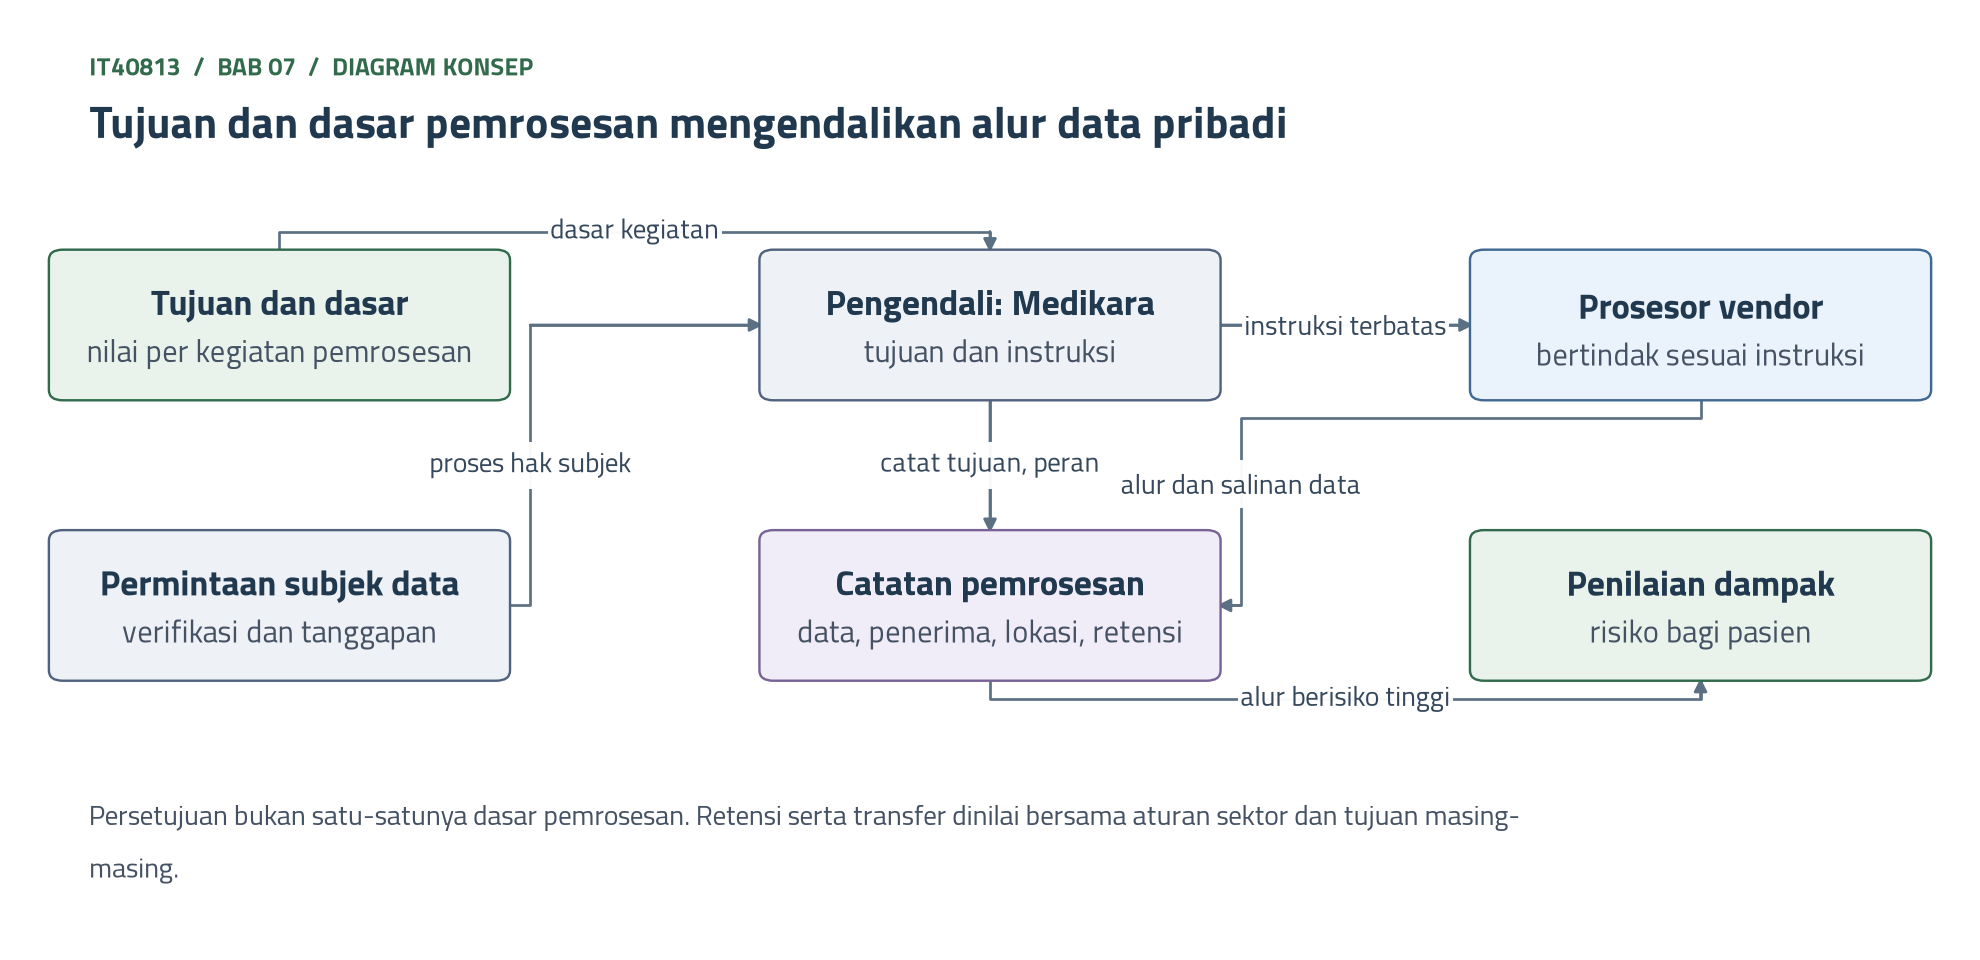
\includegraphics[width=0.96\textwidth,height=0.77\textheight,keepaspectratio]{../../figures/ch07-diagram-konsep.png}
  \label{fig:session07-ilustrasi-bab}
\end{frame}

\section{Data, Tujuan, dan Dasar}

\begin{frame}{{\Large Data Umum dan Data Spesifik}}
  \vspace{4pt}
  \footnotesize
  \begin{tabularx}{\textwidth}{|>{\raggedright\arraybackslash}X|>{\raggedright\arraybackslash}p{0.3\textwidth}|>{\raggedright\arraybackslash}X|}
    \hline
    \textbf{Data} & \textbf{Jenis menurut Pasal 4} & \textbf{Akibat pada pengelolaan} \\ \hline
    Nama dan jenis kelamin pada pendaftaran & Umum & Tetap perlu dasar, tujuan, dan pengamanan \\
    \hline
    Diagnosis, hasil laboratorium, resep & Spesifik: kesehatan & Potensi risiko tinggi, Pasal 34
    ayat (2) huruf b \\ \hline
    Nama dan poli pada janji temu & Gabungan; diperlakukan spesifik (penafsiran bab) & Akses
    dibatasi
    seperti data klinis \\ \hline
    Data pasien anak & Spesifik: data anak & Persetujuan orang tua atau wali, Pasal 25 \\ \hline
  \end{tabularx}

  \vspace{8pt}
  \small Analogi buku tamu: nama di buku tamu poli jantung sudah bercerita tentang kesehatan.
\end{frame}

\begin{frame}{{\Large Tujuan Membatasi Pemrosesan}}
  \vspace{6pt}
  \small
  \begin{itemize}
    \item Pasal 16 ayat (2): terbatas dan spesifik, sah, transparan, sesuai tujuan, aman, dapat
          dibuktikan.
    \item Analogi kunci rumah: izin memperbaiki keran bukan izin membuka seluruh lemari.
    \item 28.000 janji temu per bulan memuat nama dan poli tujuan.
    \item IT40613: 4 bidang menjadi 10 bidang menaikkan paparan 1.240 rekam dari 4.960 menjadi
          12.400 butir data.
    \item Bidang yang tidak pernah dikirim tidak dapat bocor lewat jalur itu.
  \end{itemize}
\end{frame}

\begin{frame}{{\Large Enam Dasar, Bukan Satu Kotak Persetujuan}}
  \vspace{2pt}
  \scriptsize
  \begin{tabularx}{\textwidth}{|>{\raggedright\arraybackslash}p{0.2\textwidth}|>{\raggedright\arraybackslash}X|>{\raggedright\arraybackslash}X|}
    \hline
    \textbf{Tujuan} & \textbf{Dasar kandidat (penafsiran bab)} & \textbf{Bila pasien menolak atau
    menarik} \\ \hline
    Pendaftaran janji temu & Perjanjian atau permintaan subjek data, Pasal 20 ayat (2) huruf b &
    Layanan daring tidak berjalan; pasien memakai loket \\ \hline
    Pelayanan dan rekam medis & Kewajiban hukum, huruf c; UU 17/2023 Pasal 296, PP 28/2024 Pasal 779
    & Pencatatan tetap berjalan; retensi 25 tahun tetap berlaku \\ \hline
    Gawat darurat, pasien tidak sadar & Kepentingan vital, huruf d & Persetujuan tidak dapat diminta
    saat itu \\ \hline
    Pembukaan rekam medis untuk asuransi & Persetujuan, huruf a; Permenkes 24/2022 Pasal 34 ayat (1)
    huruf c & Klaim lewat jalur itu berhenti; perlu jalur lain \\ \hline
    Promosi layanan lain & Persetujuan terpisah, huruf a & Keluar dari daftar paling lambat
    $3 \times 24$ jam \\ \hline
  \end{tabularx}

  \vspace{6pt}
  \small PP 28/2024 Pasal 963 ayat (1): persetujuan dan/atau dasar lain.
\end{frame}

\begin{frame}{{\Large Kasus Medikara: Satu Kotak untuk Tiga Tujuan}}
  \vspace{6pt}
  \small
  \begin{itemize}
    \item Misalkan satu kotak centang dipakai 336.000 janji temu per tahun. Pasal 22 ayat (4)
          meminta tujuan lain dapat dibedakan.
    \item Daftar promosi 2.000 pasien dibekukan. Misalkan 40 persen setuju kembali: 800 pasien.
    \item Bila 150 pasien menarik persetujuan, daftar 2.000 turun menjadi 1.850 dalam $3 \times 24$
          jam.
    \item Rekam medis berdasar persetujuan berbenturan dengan retensi 25 tahun.
    \item Persetujuan menuntut bukti: Pasal 24 dan Pasal 22 ayat (5).
  \end{itemize}
\end{frame}

\section{Peran}

\begin{frame}{{\Large Pengendali, Prosesor, dan Tanggung Jawab}}
  \vspace{8pt}
  \begin{center}
    \resizebox{0.97\textwidth}{!}{\begin{tikzpicture}[
  font=\scriptsize,
  simpul/.style={draw, rounded corners, align=center, minimum height=1.25cm},
  panah/.style={-{Stealth[length=2mm]}, thick},
  ket/.style={align=center, font=\tiny}]
  \node[simpul, text width=1.45cm, fill=blue!8] (pasien) at (0,0) {Pasien\\ {\tiny\mdseries subjek
    data}};
  \node[simpul, text width=2.25cm, fill=praditagreen!15] (medikara) at (3.3,0) {Medikara\\
    {\tiny\mdseries pengendali: menentukan tujuan dan kendali}};
  \node[simpul, text width=2.25cm, fill=blue!8] (vendor) at (6.7,0) {Vendor Medikara+\\
    {\tiny\mdseries prosesor: memproses atas perintah}};
  \node[simpul, text width=2.05cm, fill=blue!8] (lain) at (10.0,0) {Prosesor lain\\
    {\tiny\mdseries contoh: penyedia pendukung}};
  \node[simpul, text width=3.1cm, fill=orange!12] (tetap) at (3.3,-2.15) {Tetap pada pengendali\\
    {\tiny\mdseries mengawasi (Pasal 37), mencegah akses tidak sah (Pasal 39), memberi tahu
    (Pasal 46)}};
  \node[simpul, text width=3.1cm, fill=red!22] (luar) at (7.4,-2.15) {Di luar perintah dan tujuan\\
    {\tiny\mdseries tanggung jawab prosesor (Pasal 51 ayat (6)), bila terbukti}};
  \draw[panah] (pasien) -- node[ket, above] {data dan\\ hak} (medikara);
  \draw[panah] (medikara) -- node[ket, above] {perintah} (vendor);
  \draw[panah] (vendor) -- node[ket, above] {izin\\ tertulis} (lain);
  \draw[panah] (medikara) -- (tetap);
  \draw[panah] (vendor) -- (vendor |- luar.north);
\end{tikzpicture}
}
  \end{center}
  \vspace{4pt}
  \small Pasal 1, Pasal 51, Pasal 52. Analogi penitipan dokumen: pemilik menentukan tujuan, penyedia
  menjalankan instruksi. Penafsiran bab.
\end{frame}

\begin{frame}{{\Large Pertanyaan untuk Menentukan Tanggung Jawab}}
  \vspace{4pt}
  \footnotesize
  \begin{tabularx}{\textwidth}{|>{\raggedright\arraybackslash}X|>{\raggedright\arraybackslash}X|>{\raggedright\arraybackslash}X|}
    \hline
    \textbf{Pertanyaan} & \textbf{Bukti} & \textbf{Akibat keputusan} \\ \hline
    Siapa menentukan tujuan? & Kebijakan layanan dan keputusan bisnis & Tentukan pengendali per
    kegiatan \\ \hline
    Siapa memberi instruksi? & Kontrak serta perubahan instruksi & Batasi tindakan prosesor \\
    \hline
    Siapa melibatkan pihak lain? & Persetujuan tertulis dan daftar prosesor lain & Pasal 51 ayat (5)
    dapat diuji \\ \hline
    Siapa menangani permintaan pasien? & Alur permintaan dan catatan tanggapan & Cegah pasien
    dipingpong \\ \hline
    Siapa memberi tahu saat kegagalan? & Prosedur insiden dan bukti pengiriman & Pengendali memiliki
    data tepat waktu \\ \hline
  \end{tabularx}
\end{frame}

\begin{frame}{{\Large Kasus Medikara: Akun Dukungan di Luar Penugasan}}
  \vspace{6pt}
  \small
  \begin{itemize}
    \item Siapa bertanggung jawab atas 1.240 rekam? Bila terbukti di luar perintah, Pasal 51 ayat
          (6) mengarah ke vendor.
    \item Bukti belum lengkap: catatan hanya memuat ID aplikasi, bukan ID orang.
    \item Siapa wajib memberi tahu pasien? Pasal 46 menyebut pengendali, yaitu Medikara.
    \item Pasal 37 dan 39 tetap berlaku: 12 dari 120 akun luput dari peninjauan.
    \item Klausul 12 jam (K-05) tidak menggantikan Pasal 46. Pembacaan ini penafsiran bab.
  \end{itemize}
\end{frame}

\begin{frame}{{\Large Fungsi Pelindungan Data dan Putusan MK}}
  \vspace{6pt}
  \small
  \begin{itemize}
    \item Pasal 53 ayat (1) memuat tiga keadaan. Putusan MK 151/PUU-XXII/2024: kata ``dan'' pada
          huruf b dimaknai ``dan/atau''.
    \item Medikara: sekitar 1,2 juta kunjungan per tahun, data kesehatan sebagai kegiatan inti.
    \item Misalkan 1 petugas penuh waktu dan 5 koordinator 20 persen: setara 2 orang, 320 jam per
          bulan.
    \item Kepala TI tidak dipilih, karena ia ikut menentukan cara pemrosesan.
    \item Analogi petugas keselamatan kerja: memeriksa, tetapi tidak mengoperasikan mesin.
  \end{itemize}
\end{frame}

\section{Hak Subjek Data}

\begin{frame}{{\Large Hak, Batas, dan Bukti}}
  \vspace{2pt}
  \scriptsize
  \begin{tabularx}{\textwidth}{|>{\raggedright\arraybackslash}X|>{\raggedright\arraybackslash}p{0.17\textwidth}|>{\raggedright\arraybackslash}X|>{\raggedright\arraybackslash}p{0.15\textwidth}|>{\raggedright\arraybackslash}X|}
    \hline
    \textbf{Hak} & \textbf{Pasal} & \textbf{Batas} & \textbf{Pemilik} & \textbf{Bukti} \\ \hline
    Akses dan salinan & 7, 32 & $3 \times 24$ jam sejak diterima & Rekam medis & Tiket dan
    pengiriman \\
    \hline
    Perbaikan & 6, 30 & $3 \times 24$ jam sejak diterima & Rekam medis & Jejak perubahan \\ \hline
    Menarik persetujuan & 9, 40 & $3 \times 24$ jam sejak diterima & Pemasaran & Daftar sebelum dan
    sesudah \\ \hline
    Menunda atau membatasi & 11, 41 & $3 \times 24$ jam sejak diterima & Fungsi privasi & Pengaturan
    sistem \\ \hline
    Mengakhiri dan menghapus & 8, 42, 43, 44 & Tanpa rentang jam; mengikuti peraturan & Fungsi
    privasi & Keputusan dan alasan \\ \hline
  \end{tabularx}

  \vspace{6pt}
  \small Analogi loket berkas: nomor antrean, periksa identitas, nilai, simpan tanda terima.
\end{frame}

\begin{frame}{{\Large Dua Contoh: Beban dan Penghapusan}}
  \vspace{6pt}
  \small
  \begin{itemize}
    \item Misalkan 0,1 persen dari 28.000 janji temu: 28 permintaan per bulan, 45 menit per
          permintaan.
    \item Beban 21 jam per bulan, 252 jam per tahun, sekitar 1,6 bulan kerja.
    \item Permintaan Jumat 16.00 selesai Senin 16.00. Loket Senin sampai Jumat hanya punya 9 jam
          kerja.
    \item Pasien terakhir berkunjung 2 Maret 2026: rekam medis paling singkat sampai 2 Maret 2051.
    \item Hapus dari daftar promosi, jelaskan alasan rekam medis tidak dihapus, catat keduanya.
  \end{itemize}
\end{frame}

\section{Catatan Pemrosesan}

\begin{frame}{{\Large Catatan Pemrosesan: Satu Baris per Kegiatan}}
  \vspace{6pt}
  \small
  \begin{itemize}
    \item Pasal 31: pengendali merekam seluruh kegiatan pemrosesan. RoPA adalah nama lembar kerja.
    \item Analogi kartu persediaan: asal, tujuan, lokasi, dan masa simpan barang.
    \item Catatan dukungan 90 hari: sekitar 84.000 baris. Disalin 25 tahun: 8,4 juta baris,
          100 kali.
    \item 6 proses pada 36 fasilitas: 216 baris atau 144 jam. Dikelompokkan: 28 baris,
          sekitar 19 jam.
    \item Salinan pihak ketiga PP 33/2026 Pasal 74 menyebut 13 butir: dipantau, belum kewajiban.
  \end{itemize}
\end{frame}

\begin{frame}{{\Large Contoh Catatan Pemrosesan (Misalkan)}}
  \vspace{2pt}
  \scriptsize
  \begin{tabularx}{\textwidth}{|>{\raggedright\arraybackslash}p{0.15\textwidth}|>{\raggedright\arraybackslash}X|>{\raggedright\arraybackslash}X|>{\raggedright\arraybackslash}X|}
    \hline
    \textbf{Butir} & \textbf{P-01 Pendaftaran} & \textbf{P-02 Telekonsultasi} & \textbf{P-05
    Dukungan vendor} \\ \hline
    Tujuan, pemilik & Janji temu; pemilik Medikara+ & Pelayanan jarak jauh; pemilik rekam medis &
    Perbaikan gangguan; pengelola vendor \\ \hline
    Data & Identitas, poli, jadwal & Keluhan dan catatan klinis & Data tiket; akses baca terbatas \\
    \hline
    Dasar & Perjanjian, huruf b & Kewajiban hukum, huruf c & Perjanjian; instruksi tertulis \\
    \hline
    Penerima & Vendor sesuai instruksi & Tenaga kesehatan berwenang & Staf vendor yang ditugaskan \\
    \hline
    Lokasi & Harus dikonfirmasi & Pusat data dalam negeri & Harus dikonfirmasi \\ \hline
    Retensi & Ditetapkan per tujuan & Mengikuti rekam medis & 90 hari \\ \hline
    Bukti & Dasar, instruksi, akses & Dasar, akses, jejak perubahan & AC-01 dan daftar 120 akun \\
    \hline
  \end{tabularx}
\end{frame}

\begin{frame}{{\Large Dua Masa Simpan yang Sering Tertukar}}
  \vspace{6pt}
  \small
  \begin{itemize}
    \item Rekam medis: paling singkat 25 tahun sejak kunjungan terakhir, Permenkes 24/2022 Pasal 39.
    \item Catatan akses: berapa lama organisasi dapat membuktikan siapa membaca apa.
    \item Catatan rinci 7 hari, diketahui hari ke-11: 620 rekam terlacak, 620 rekam tinggal jumlah.
    \item Pasal 46 ayat (2) huruf a meminta data yang terungkap. Separuh rekam tidak dapat dijawab.
    \item Dinaikkan menjadi 90 hari: ruang simpan sekitar 12,9 kali, dan perlu baris RoPA sendiri.
  \end{itemize}
\end{frame}

\section{Lokasi dan Transfer}

\begin{frame}{{\Large Lokasi dan Transfer: Dua Lapis Aturan}}
  \vspace{2pt}
  \begin{center}
    \resizebox{!}{0.66\textheight}{\begin{tikzpicture}[
  tanya/.style={draw, rounded corners, align=center, text width=1.62cm, minimum height=1.95cm,
    font=\scriptsize, fill=orange!12},
  mulai/.style={draw, rounded corners, align=center, text width=7.4cm, minimum height=0.7cm,
    font=\scriptsize, fill=blue!8},
  henti/.style={draw, rounded corners, align=center, text width=1.62cm, minimum height=1.45cm,
    font=\scriptsize, fill=red!22},
  perbaiki/.style={draw, rounded corners, align=center, text width=1.62cm, minimum height=1.45cm,
    font=\scriptsize, fill=gray!35},
  hasil/.style={draw, rounded corners, align=center, text width=1.62cm, minimum height=1.45cm,
    font=\scriptsize, fill=green!10},
  ket/.style={font=\tiny, inner sep=1pt},
  panah/.style={-{Stealth[length=2mm]}, thick}]
  \node[mulai, anchor=west] (awal) at (-0.92,1.65) {Usulan: data pasien disimpan, dikirim, atau
    ditampilkan ke luar wilayah Indonesia};
  \node[tanya] (a) at (0,0) {Data kesehatan atau rekam medis?\\ {\tiny\mdseries PP 28/2024 Pasal
    966, 972}};
  \node[tanya] (b) at (2.35,0) {Penyimpanan rutin di luar negeri?\\ {\tiny\mdseries Pasal 966 ayat
    (2), ayat (5)}};
  \node[tanya] (c) at (4.7,0) {Tujuan spesifik dan terbatas?\\ {\tiny\mdseries Pasal 972 ayat (2)}};
  \node[tanya] (d) at (7.05,0) {Izin Menteri sudah ada?\\ {\tiny\mdseries Pasal 972 ayat (3) huruf
    a}};
  \node[tanya] (e) at (9.4,0) {Syarat transfer terpenuhi?\\ {\tiny\mdseries UU PDP Pasal 56 ayat (2)
    sampai (4)}};
  \node[perbaiki] (a2) at (0,-2.55) {Baca UU PDP Pasal 56 dan PP 71/2019 Pasal 21};
  \node[henti] (b2) at (2.35,-2.55) {Berhenti: pusat data wajib di dalam Indonesia};
  \node[henti] (c2) at (4.7,-2.55) {Berhenti: rancang ulang alur data};
  \node[perbaiki] (d2) at (7.05,-2.55) {Ajukan izin sebelum transfer};
  \node[hasil] (e2) at (9.4,-2.55) {Jalan dengan bukti\\ {\tiny\mdseries bila tidak terpenuhi:
    berhenti}};
  \draw[panah] (a |- awal.south) -- (a);
  \draw[panah] (a) -- node[ket, above] {Ya} (b);
  \draw[panah] (b) -- node[ket, above] {Tidak} (c);
  \draw[panah] (c) -- node[ket, above] {Ya} (d);
  \draw[panah] (d) -- node[ket, above] {Ya} (e);
  \draw[panah] (a) -- node[ket, right] {Tidak} (a2);
  \draw[panah] (b) -- node[ket, right] {Ya} (b2);
  \draw[panah] (c) -- node[ket, right] {Tidak} (c2);
  \draw[panah] (d) -- node[ket, right] {Tidak} (d2);
  \draw[panah] (e) -- node[ket, right] {Ya} (e2);
\end{tikzpicture}
}
  \end{center}
  \vspace{-6pt}
  \small Urutan pertanyaan adalah penafsiran bab.
\end{frame}

\begin{frame}{{\Large Dua Contoh: Penawaran Murah dan Dukungan Jarak Jauh}}
  \vspace{6pt}
  \small
  \begin{itemize}
    \item Bab 3: penawaran luar negeri Rp420 juta, hemat Rp180 juta atau 30 persen dari Rp600 juta.
    \item Persetujuan pasien pada Pasal 56 tidak menjawab Pasal 966 ayat (2) PP 28/2024.
    \item Misalkan 4 staf vendor di luar negeri membuka layar untuk sekitar 300 tiket per bulan.
    \item Pasal 971 ayat (2) menyebut penampilan sebagai bentuk transfer (penafsiran bab).
    \item Dukungan dalam negeri misalkan lebih mahal Rp25 juta per bulan, atau Rp300 juta per tahun.
  \end{itemize}
\end{frame}

\section{Penilaian Dampak}

\begin{frame}{{\Large Penyaringan Tiga Usulan terhadap Pasal 34 Ayat (2)}}
  \vspace{2pt}
  \scriptsize
  \begin{tabularx}{\textwidth}{|>{\raggedright\arraybackslash}p{0.3\textwidth}|>{\raggedright\arraybackslash}X|>{\raggedright\arraybackslash}X|>{\raggedright\arraybackslash}X|}
    \hline
    \textbf{Keadaan} & \textbf{Klaim asuransi} & \textbf{Triase otomatis} & \textbf{Tampilan
    baru} \\
    \hline
    a. Keputusan otomatis & Tidak & Ya & Tidak \\ \hline
    b. Data spesifik & Ya & Ya & Sudah ada, tidak berubah \\ \hline
    c. Skala besar & Ya: 72.000 per tahun & Perlu dihitung & Sudah ada, tidak berubah \\ \hline
    d. Evaluasi atau pemantauan & Tidak & Ya: penskoran gejala & Tidak \\ \hline
    e. Penggabungan data & Ya & Tidak & Tidak \\ \hline
    f. Teknologi baru & Tidak & Ya & Tidak \\ \hline
    g. Membatasi hak & Perlu diperiksa & Perlu diperiksa & Tidak \\ \hline
    \textbf{Keputusan} & DPIA sebelum aktif & DPIA sebelum uji coba & Tinjau DPIA lama bila alur
    berubah \\ \hline
  \end{tabularx}
\end{frame}

\begin{frame}{{\Large DPIA: Risiko bagi Pasien, Bukan Hanya Organisasi}}
  \vspace{6pt}
  \small
  \begin{itemize}
    \item Analogi ruang operasi baru: pemeriksaan dilakukan sebelum pasien masuk.
    \item 5 dari 6 proses memuat data kesehatan: 5 kali 72 jam, atau 360 jam dan Rp21,6 juta.
    \item Pembanding WP 248 rev.01: dua kriteria pada umumnya perlu DPIA. Pasal 34 tidak memuat
          aturan itu.
    \item R-01 berskor $3 \times 4 = 12$ dan Rp100 juta per tahun. Itu risiko bagi organisasi.
    \item Satu rekam poli kejiwaan terungkap: dampak 1 bagi Medikara, tetapi stigma bagi pasien.
  \end{itemize}
\end{frame}

\section{Pemberitahuan}

\begin{frame}{{\Large Pasal 46: Isi Kewajiban}}
  \vspace{6pt}
  \small
  \begin{itemize}
    \item Ayat (1): pemberitahuan tertulis paling lambat $3 \times 24$ jam kepada subjek data
          dan lembaga.
    \item Ayat (2): data terungkap, kapan dan bagaimana, serta penanganan dan pemulihan.
    \item Ayat (3): kepada masyarakat dalam hal tertentu.
    \item Contoh dasar: kegagalan dan penemuan bersamaan Jumat 20.00, batas Senin 20.00 WIB.
    \item Varian Bab 3: vendor melapor setelah 30 jam, kontrak terlewati 18 jam, sisa 42 jam.
  \end{itemize}
\end{frame}

\begin{frame}{{\Large Alur Keputusan Insiden}}
  \vspace{16pt}
  \begin{center}
    \resizebox{0.9\textwidth}{!}{\begin{tikzpicture}[
  font=\scriptsize,
  tahap/.style={draw, rounded corners, align=center, text width=2.25cm,
    minimum height=1.45cm, fill=blue!8},
  panah/.style={-{Stealth[length=2mm]}, thick}]
  \node[tahap] (n0) at (0,0) {Temukan\\dan amankan\\ {\tiny\mdseries catat dua waktu}};
  \node[tahap, fill=orange!12] (n1) at (2.8,0) {Nilai data\\serta waktu\\ {\tiny\mdseries pisahkan
    pasti dan sementara}};
  \node[tahap] (n2) at (5.6,0) {Putuskan\\dan beri tahu\\ {\tiny\mdseries subjek data dan lembaga}};
  \node[tahap, fill=green!10] (n3) at (8.4,0) {Pulihkan\\dan perbaiki\\ {\tiny\mdseries bukti dan
    uji ulang}};
  \draw[panah] (n0) -- (n1);
  \draw[panah] (n1) -- (n2);
  \draw[panah] (n2) -- (n3);
\end{tikzpicture}
}
  \end{center}
  \vspace{10pt}
  \small Analogi peringatan kerusakan produk: menunggu seluruh penyebab membuat pengguna terus
  terpapar. Waktu kejadian dan waktu diketahui dicatat terpisah.
\end{frame}

\begin{frame}{{\Large Kapan Rentang 72 Jam Mulai Dihitung?}}
  \vspace{6pt}
  \small
  \begin{itemize}
    \item Pasal 46 ayat (1) tidak menulis titik mulai. Pasal 30, 32, 40, dan 41 menulis ``terhitung
          sejak''.
    \item Salinan pihak ketiga PP 33/2026 Pasal 114 ayat (2): ``diketahui secara pasti, patut, dan
          wajar''. Naskah resmi belum diperoleh; mulai berlaku 16 Januari 2027. Hanya dipantau.
    \item GDPR dan EDPB: tingkat kepastian yang wajar. Hanya pembanding.
    \item Sikap kerja (penafsiran bab): batas terluar dihitung dari saat pertama diketahui.
    \item Fungsi hukum, pemilik R-12, menetapkan batas operasional konservatif.
  \end{itemize}
\end{frame}

\begin{frame}{{\Large Insiden 2025: Tiga Pembacaan Rentang 72 Jam}}
  \vspace{2pt}
  \begin{center}
    \resizebox{0.97\textwidth}{!}{\begin{tikzpicture}[
  font=\scriptsize,
  x=0.82cm,
  batang/.style={draw, rounded corners=1pt, minimum height=0.6cm, align=center, inner sep=1pt,
    font=\tiny},
  ket/.style={align=center, font=\tiny},
  panah/.style={-{Stealth[length=2mm]}, thick}]
  % Sumbu hari: satu satuan x sama dengan satu hari, hari ke-1 berada pada x = 1.
  \draw[panah] (0.7,0) -- (14.6,0);
  \foreach \hari/\nama in {1/Selasa, 4/Jumat, 8/Selasa, 11/Jumat, 14/Senin} {
    \draw[thick] (\hari,0.1) -- (\hari,-0.1);
    \node[ket] at (\hari,-0.45) {Hari \hari\\ \nama};
  }
  % Lapisan fakta latihan: rekam kunjungan dan catatan rinci.
  \node[batang, fill=red!22, text width=3.2cm, anchor=west] at (1,1.15)
    {Malam 1 sampai 4: 620 rekam, hanya jumlah};
  \node[batang, fill=green!10, text width=3.2cm, anchor=west] at (5,1.15)
    {Malam 5 sampai 8: 620 rekam terlacak};
  \node[batang, fill=gray!35, text width=4.85cm, anchor=west] at (5,0.46)
    {Catatan rinci tersisa saat diketahui: 7 hari};
  \node[ket, anchor=west] at (11.2,1.05) {Keluhan pasien\\ hari 11, 20.00 WIB};
  \draw[thick, dashed] (11,0.1) -- (11,1.4);
  % Tiga pembacaan rentang 72 jam.
  \draw[panah, blue!60!black] (1,-1.05) -- (4,-1.05);
  \node[ket, anchor=west] at (4.15,-1.05) {dari panggilan pertama: batas hari 4, lewat sebelum
    diketahui};
  \draw[panah, orange!70!black] (8,-1.65) -- (11,-1.65);
  \node[ket, anchor=east] at (7.85,-1.65) {dari panggilan terakhir: batas tepat saat diketahui};
  \draw[panah, green!40!black] (11,-2.25) -- (14,-2.25);
  \node[ket, anchor=east] at (10.85,-2.25) {dari saat diketahui: batas Senin 20.00 WIB};
\end{tikzpicture}
}
  \end{center}
  \vspace{-4pt}
  \small Dari panggilan pertama, batas lewat 168 jam sebelum Medikara tahu. Jam adalah pengandaian.
\end{frame}

\begin{frame}{{\Large Jam-Jam Pertama: Angka Belum Pasti}}
  \vspace{6pt}
  \begin{center}
    \resizebox{0.97\textwidth}{!}{\begin{tikzpicture}[
  font=\scriptsize,
  kotak/.style={draw, rounded corners, align=center, text width=2.9cm, minimum height=1.2cm},
  jam/.style={align=center, font=\tiny},
  panah/.style={-{Stealth[length=2mm]}, thick}]
  % Skala garis tidak proporsional. Jam dihitung dari saat Medikara mengetahui kejadian.
  \draw[panah] (-0.3,0) -- (10.0,0);
  \foreach \posisi in {0, 1.85, 3.7, 5.55, 7.4, 9.25}
    \draw[thick] (\posisi,0.1) -- (\posisi,-0.1);
  \node[kotak, fill=red!22] (a) at (0,1.15) {Keluhan pasien sampai ke koordinator. Jumlah belum
    diketahui};
  \node[kotak, fill=blue!8] (b) at (1.85,-1.45) {Vendor mengakui akun masih aktif. Akun
    dinonaktifkan};
  \node[kotak, fill=orange!12] (c) at (3.7,1.15) {Rekap harian: jumlah sementara 1.240 rekam};
  \node[kotak, fill=orange!12] (d) at (5.55,-1.45) {620 rekam terlacak, 620 rekam tinggal jumlah};
  \node[kotak, fill=blue!8] (e) at (7.4,1.15) {Akar sebab belum selesai. Pemberitahuan tidak
    menunggu};
  \node[kotak, fill=green!10] (f) at (9.25,-1.45) {Batas terluar kerja bila dihitung dari saat
    diketahui};
  \draw (a) -- (0,0.1);
  \draw (b) -- (1.85,-0.1);
  \draw (c) -- (3.7,0.1);
  \draw (d) -- (5.55,-0.1);
  \draw (e) -- (7.4,0.1);
  \draw (f) -- (9.25,-0.1);
  \node[jam, fill=white, inner sep=1pt] at (0,-0.38) {Jam 0\\ Jumat 20.00};
  \node[jam, fill=white, inner sep=1pt] at (1.85,0.38) {Jam 1\\ Jumat 21.00};
  \node[jam, fill=white, inner sep=1pt] at (3.7,-0.38) {Jam 12\\ Sabtu 08.00};
  \node[jam, fill=white, inner sep=1pt] at (5.55,0.38) {Jam 18\\ Sabtu 14.00};
  \node[jam, fill=white, inner sep=1pt] at (7.4,-0.38) {Jam 40\\ Minggu 12.00};
  \node[jam, fill=white, inner sep=1pt] at (9.25,0.38) {Jam 72\\ Senin 20.00};
\end{tikzpicture}
}
  \end{center}
  \small Jumlah sementara tersedia pada jam ke-12. Pada jam ke-18, 25 persen rentang sudah terpakai.
\end{frame}

\begin{frame}{{\Large Kasus Medikara: Isi Pemberitahuan Senin Pagi}}
  \vspace{4pt}
  \footnotesize
  \begin{tabularx}{\textwidth}{|>{\raggedright\arraybackslash}p{0.2\textwidth}|>{\raggedright\arraybackslash}X|>{\raggedright\arraybackslash}X|}
    \hline
    \textbf{Unsur Pasal 46 ayat (2)} & \textbf{Sudah pasti} & \textbf{Sementara atau belum
    diketahui} \\ \hline
    Data yang terungkap & Rekam kunjungan pada dua rumah sakit & Jumlah 1.240 dari rekap; 620 rekam
    belum terhubung ke nama \\ \hline
    Kapan dan bagaimana & 8 malam, lewat akun dukungan vendor yang aktif setelah kontrak selesai &
    Orang yang memakai akun; apakah data disalin keluar \\ \hline
    Penanganan dan pemulihan & Akun dinonaktifkan; 120 akun diperiksa & Akar sebab; hasil
    pemeriksaan di sisi vendor \\ \hline
  \end{tabularx}

  \vspace{8pt}
  \small Tim tidak menunggu angka final. Cara bertahap dicatat bersama fungsi hukum.
\end{frame}

\begin{frame}{{\Large Kasus Medikara: 620 Rekam yang Tidak Terlacak}}
  \vspace{4pt}
  \footnotesize
  \begin{tabularx}{\textwidth}{|>{\raggedright\arraybackslash}X|>{\raggedright\arraybackslash}p{0.27\textwidth}|>{\raggedright\arraybackslash}X|}
    \hline
    \textbf{Pilihan} & \textbf{Biaya langsung} & \textbf{Kelemahan} \\ \hline
    A. Hanya 620 pasien terlacak & Rp9,3 juta & 620 rekam lain tanpa pemberitahuan \\ \hline
    B. A, pengumuman, dan kanal tanya jawab & Rp9,3 juta ditambah Rp4,8 juta: Rp14,1 juta & Pesan
    umum tidak menjamin terbaca \\ \hline
    C. Pesan ke seluruh kunjungan dua rumah sakit & 360.000 pesan kali Rp500: Rp180 juta & Sebagian
    besar tidak terdampak \\ \hline
  \end{tabularx}

  \vspace{8pt}
  \small Misalkan tim mengusulkan B: biaya langsung naik dari Rp23,7 juta menjadi Rp28,5 juta.
  Fungsi hukum menilai Pasal 46 ayat (3).
\end{frame}

\begin{frame}{{\Large Membaca Dua Penelitian}}
  \vspace{6pt}
  \small
  \begin{itemize}
    \item McCoy dan Perlis (2018): 2.149 pelanggaran, 176,4 juta rekam di Amerika Serikat, 2010
          sampai 2017.
    \item Penyedia layanan: 70 persen pelanggaran, 21 persen rekam. \textit{Health plan}: 13 persen
          dan 63 persen.
    \item Choi dan rekan (2019): 3.025 rumah sakit. Sesudah pelanggaran, waktu sampai
          elektrokardiogram naik hingga 2,7 menit.
    \item Mortalitas 30 hari infark miokard akut naik hingga 0,36 poin persentase. Ini asosiasi.
    \item Angka tidak disalin ke Medikara. Kontrol baru diuji dampaknya pada pelayanan klinis.
  \end{itemize}
\end{frame}

\section{Status, Sanksi, dan Sistem}

\begin{frame}{{\Large Status Sumber Hukum per 1 November 2026}}
  \vspace{2pt}
  \scriptsize
  \begin{tabularx}{\textwidth}{|>{\raggedright\arraybackslash}p{0.24\textwidth}|>{\raggedright\arraybackslash}X|>{\raggedright\arraybackslash}X|}
    \hline
    \textbf{Sumber} & \textbf{Status kerja} & \textbf{Tindakan} \\ \hline
    UU 27/2022 & Naskah resmi terbaca; Pasal 74 berakhir 17 Oktober 2024 & Turunkan kewajiban serta
    bukti \\ \hline
    Putusan MK 151/PUU-XXII/2024 & Amar resmi terbaca & Baca bersama Pasal 53 \\ \hline
    PP 28/2024; Permenkes 24/2022 & Naskah resmi terbaca & Turunkan kewajiban sektor \\ \hline
    PP 33/2026 & Salinan pihak ketiga dan ringkasan; naskah resmi belum diperoleh & Pantau; jangan
    menetapkan pasal sebagai kewajiban \\ \hline
    Perpres dan lembaga & Berita Juli dan September 2026; naskah belum ditemukan & Tetapkan
    penanggung jawab kanal \\ \hline
    Peraturan lembaga & Belum ditemukan & Pantau \\ \hline
  \end{tabularx}

  \vspace{6pt}
  \small Analogi jadwal perjalanan: pengumuman rute baru belum berarti jadwal dapat dipesan.
\end{frame}

\begin{frame}{{\Large Sanksi dan Masa Penyesuaian}}
  \vspace{6pt}
  \small
  \begin{itemize}
    \item Pasal 57: peringatan, penghentian sementara, penghapusan, dan denda paling tinggi
          2 persen.
    \item Misalkan variabel Rp500 miliar: paling tinggi Rp10 miliar, sekitar 422 kali Rp23,7 juta.
          Alat diskusi, bukan perkiraan.
    \item Pasal 67 ayat (1): 5 tahun dan/atau Rp5 miliar, dengan unsur sengaja dan melawan hukum.
    \item Pasal 74 berakhir 17 Oktober 2024. Insiden 2025 tidak punya alasan ``masih masa
          penyesuaian''.
    \item PP 33/2026 berlaku 2027, sehingga tidak dipakai menilai kejadian 2025 (penafsiran bab).
  \end{itemize}
\end{frame}

\begin{frame}{{\Large Sistem Manajemen Privasi dan Celah C2}}
  \vspace{6pt}
  \small
  \begin{itemize}
    \item ISO/IEC 27701:2025 tentang PIMS kini standar mandiri. Sertifikat tidak menggantikan
          analisis dasar.
    \item Uji sampel: 12 dari 150 pasien yang menarik persetujuan masih menerima promosi, 8 persen.
    \item Kode CP-01 sampai CP-07 melanjutkan G-01 sampai G-06. Tabel lengkap ada pada modul.
    \item Misalkan tiga prioritas: CP-04 pemberitahuan, CP-01 perjanjian vendor, CP-05
          catatan rinci.
    \item Latihan pemberitahuan dua kali setahun: 12 orang, 4 jam, atau 96 jam dan Rp5,76 juta.
  \end{itemize}
\end{frame}

\section{Aktivitas, Ringkasan, dan Latihan}

\begin{frame}{{\Large Aktivitas: Peran dan Langkah}}
  \vspace{6pt}
  \small
  \begin{itemize}
    \item Analis regulasi memimpin. Pemilik konteks memetakan alur. Analis teknologi menelusuri
          sistem. Analis risiko memperbarui R-01 dan R-12.
    \item Isi catatan pemrosesan untuk pendaftaran atau telekonsultasi, lalu uji lokasi datanya.
    \item Saring proses dengan tujuh keadaan Pasal 34.
    \item Susun kronologi, isi analisis celah, dan buat rancangan pemberitahuan yang tidak dikirim.
    \item Rangkum Bab 4 sampai 7 menjadi C2, lalu bawa tiga celah ke C3.
  \end{itemize}
\end{frame}

\begin{frame}{{\Large Aktivitas: Luaran, C2, dan Berkas}}
  \vspace{6pt}
  \small
  \begin{itemize}
    \item Luaran: RoPA, penyaringan DPIA, analisis insiden, rancangan pemberitahuan, celah PDP.
    \item Tonggak C2 Kondisi Saat Ini, ditinjau menjelang UTS.
    \item Rubrik: dasar dan peran 30 persen, alur 25 persen, kronologi dan tenggat 30 persen, bukti
          15 persen.
    \item Berkas di \berkas{sources/chapter07}: \texttt{catatan-pemrosesan.csv},
          \texttt{analisis-celah-pdp.md}, \texttt{kronologi-insiden-vendor-2025.md},
          \texttt{templat-notifikasi.md}, dan lainnya.
    \item Data nyata wajib berizin dan dianonimkan. Data pasien tidak boleh dipakai.
  \end{itemize}
\end{frame}

\begin{frame}{{\Large Ringkasan}}
  \vspace{6pt}
  \small
  \begin{itemize}
    \item Pasal 20 menyediakan enam dasar. Persetujuan hanya salah satunya.
    \item Peran dinilai per kegiatan. Kewajiban memberi tahu tetap pada pengendali.
    \item RoPA memperlihatkan alur data. Pasal 966 dan 972 PP 28/2024 dibaca bersama Pasal 56.
    \item DPIA menilai akibat bagi pasien sebelum alur berjalan.
    \item Pasal 46 tidak menulis titik mulai. Dua waktu dicatat, dan angka sementara disebut
          sementara.
  \end{itemize}
\end{frame}

\begin{frame}{{\Large Latihan}}
  \vspace{6pt}
  \small
  \begin{enumerate}
    \item Medikara memakai vendor untuk aplikasi Medikara+. Dalam hubungan ini, siapa pengendali dan
          siapa prosesor? Apa akibatnya terhadap tanggung jawab saat terjadi kebocoran?
    \item Tentukan dasar pemrosesan yang paling tepat untuk data rekam medis dalam layanan
          pengobatan. Jelaskan mengapa persetujuan belum tentu menjadi dasar yang terbaik.
    \item Susun garis waktu notifikasi yang memenuhi UU PDP untuk insiden yang ditemukan pada Jumat
          malam.
  \end{enumerate}

  \vspace{6pt}
  Tabel contoh dan lembar isian tersedia pada modul.
\end{frame}

\begin{frame}{{\Large Bacaan dan Pesan Utama}}
  \vspace{6pt}
  \small
  \href{https://peraturan.bpk.go.id/Details/229798/uu-no-27-tahun-2022}{UU 27/2022},
  \href{https://s.mkri.id/simpp/ds/6889d006383b1.pdf}{Putusan MK 151/PUU-XXII/2024},
  \href{https://peraturan.bpk.go.id/Details/294077}{PP 28/2024},
  \href{https://peraturan.bpk.go.id/Details/245544}{Permenkes 24/2022}\par
  \href{https://ec.europa.eu/newsroom/article29/items/611236}{WP 248 rev.01},
  \href{https://doi.org/10.1001/jama.2018.9222}{McCoy dan Perlis (2018)},
  \href{https://doi.org/10.1111/1475-6773.13203}{Choi dan rekan (2019)}\par
  \vspace{14pt}
  \begin{center}
    \large\textbf{Organisasi harus dapat menunjukkan alasan pemrosesan, kendali alur data, dan bukti
    pertanggungjawabannya.}
  \end{center}
\end{frame}

\end{document}
